\section{Realisierung des Prototyps}
Als Umgebung, um die Infrastruktur für den Prototypen bereitzustellen, hat der Autor das Kennenlernangebot von AWS, ein einjähriges kostenloses Kontingent an Services und Produkten \cite{FreeTier2020}, gewählt.

Nachdem der erwähnte \emph{AWS Account} erstellt war, mussten erste Schritte, wie grundlegende Konfigurationen des Identity Access Management (IAM) gemacht und das Steuern von Spot Anfragen, das Einrichten eines Container Repositories (ECR), das Aufsetzen eines öffentlich zugänglichen S3 Buckets und anderes aus dem AWS Produktekatalog, erlernt werden.

Weitere Schritte folgten. Die eigentliche Realisierung des Prototypen wird in den folgenden Kapiteln beschrieben werden. Das Endresultat wird jedoch der Nachvollziehbarkeit halber schon einmal hier abgebildet:

\begin{figure}[H]
	\centering
	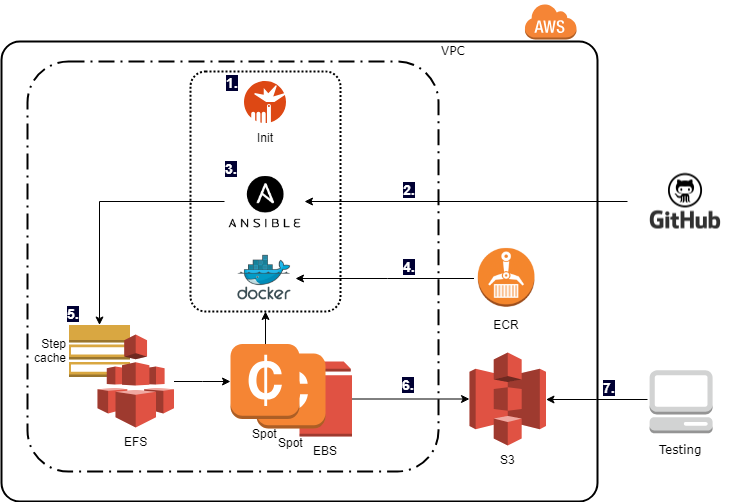
\includegraphics[width=.90\textwidth]{poc_zustand}
	\caption{Geodatenverarbeitung mit SPOT Instanzen.}
	\label{fig:ist_zustand}
\end{figure}

\subsection{Spot Flottenanfrage}
Als Setup für die Spot Flottenanfrage wurde ein sogenanntes Launch Template mit den wichtigsten Konfigurationen wie Sicherheitsgruppe, Wahl des AMI und User Data angelegt. Anschliessend wurde eine Spot Flottenanfrage basierend auf diesem Template erstellt. Wobei als Mindestanforderung an den Rechner 16 CPUs und 60 GB Memory waren. Als Option wurde gewählt, dass die Zielkapazität aufrechterhalten bleiben soll\footnote{Die Zielkapazität soll immer 1 sein.}: Somit wird nach jedem Interrupt automatisch eine neue Instanz mit der definierten Konfiguration zur Verfügung gestellt.

\subsection{Handling der Interrupts}
Wie im Kapitel \ref{kap:bugdet_instanzen} beschrieben, sind Spot Instanzen so günstig, weil sie einem jederzeit weggenommen werden können, um einem anderen Kunden zur Verfügung zu stellen. Also muss die Datenverarbeitung mit dem Handling von Interrupts umgehen können. 
Der Einfachheit halber hat der Autor gänzlich auf das \textit{Horchen eines bevorstehenden Interrupts} via RESTful Abfrage (In Anhang \ref{appendix:restful} beschrieben) oder \emph{CloudWatch} verzichtet und hat stattdessen die Datenverarbeitung als Serie betrachtet und in Schritte unterteilt. Sobald ein Schritt erledigt wird, wird dies auf dem EFS Volumen in einer Textdatei festgehalten. Falls es zu einem Interrupt kommen sollte, wird von der Spot Flotte die nächste Instanz bereitgestellt und die Publizierung macht bei dem Schritt weiter, der zuletzt in der Textdatei festgehalten wurde (Abbildung \ref{fig:ist_zustand}, Nr. 5).

\subsection{Die Datenverarbeitung als Code}
Mit der Entscheidung, die Spot Instanz via \emph{Cloud-Init}-Ansatz (Abb. \ref{fig:ist_zustand}, Nr. 1) mit Ansible zu Provisionieren\footnote{Und nicht mit einem neuen AMI.}, lag es auf der Hand, auch gleich dieselbe Technologie für die Realisierung der Datenverarbeitung zu verwenden (Nr. 3). 
Viele Annehmlichkeiten, wie die Nähe zur Shell und Python, das Logging und deklarativer Code zeigten sich in der Realisierung als hilfreich. Das Init-Skript wie auch das Ansible Playbook können auf \href{https://github.com/bfh-semesterarbeit/up-and-running-dataprocessing}{github.com/bfh-semesterarbeit} eingesehen werden.


\subsection{Testen der Datenstruktur}
Wie in Kapitel auch schon vorgekommen, dass die gelieferten Rohdaten Fehler in der Datenstruktur verwiesen.

\subsection{Monitoring}
Bezüglich Monitoring hat die Zeit nicht gereicht. Bisher wird die Datenverarbeitung lediglich geloggt. Die verwendeten Tools (der well-formed XML Test und der Output des Containers) wie auch Ansible loggen in ein Verzeichnis im EFS, das gut zugänglich ist. Vor allem die Logdatei von Ansible ist ausführlich und macht eine Fehlersuche einfach.

Um die Last des Servers zu überprüfen, wurde lediglich die Amazon Webconsole verwendet.


\subsection{Inhaltliche Kontrolle der publizierten Daten}
Das Resultat kann vorläufig\footnote{Bis am 1. November 2020} hier betrachtet werden:
\href{https://codepen.io/rebert/pen/ExKZmmE}{https://codepen.io/rebert/pen/ExKZmmE} Wobei nur die Gebäude vom S3 Testbucket kommen (Abb. \ref{fig:ist_zustand}, Nr. 7) 

\subsection{Testen}
Da es sich um eine Datenverarbeitung und nicht um einen Dienst handelt, wurde auf End-to-end Testing und Unit-Tests verzichtet. Es wurden lediglich Erfahrungen gesammelt, zum sehen, ob die Datenverarbeitung auf Spot Instanzen funktioniert. Hierzu wurden zwei Arten von Tests gemacht:

\subsubsection{Unerwartete Interrupts}
Da es in der ganzen Entwicklungsphase zu keinem einzigen Interrupt einer Spot Instanz gekommen ist, musste die Stabilität des Datenverarbeitungsprozesses auf unerwartete Interrupts manuell getestet werden. Um die Testphasen zu verkürzen, wurde die Menge der Eingangsdaten beschränkt\footnote{Auf ein Schweizerischer Kartenblatt 1:25'000.}.

Dieser Test wurde iterativ umgesetzt und der Code wurde bei Fehlern fortlaufend angepasst. 


\subsubsection{Full-load test}
Der komplette Rohdatensatz, alle (erfassten) Gebäude der Schweiz, wurde verarbeitet. Dieser Test war sozusagen die Probe aufs Exempel. Bezüglich Anforderungen an die Rechnerleistung konnte auf Erfahrungswerte aufgebaut werden.

Dabei hat dem Autoren ein einziges von den ca. 8 Millionen Gebäuden einen Streich gespielt und so trotz gewonnener Zeit in der Automatisierung 

